
%% bare_conf.tex
%% V1.4
%% 2012/12/27
%% by Michael Shell
%% See:
%% http://www.michaelshell.org/
%% for current contact information.
%%
%% This is a skeleton file demonstrating the use of IEEEtran.cls
%% (requires IEEEtran.cls version 1.8 or later) with an IEEE conference paper.
%%
%% Support sites:
%% http://www.michaelshell.org/tex/ieeetran/
%% http://www.ctan.org/tex-archive/macros/latex/contrib/IEEEtran/
%% and
%% http://www.ieee.org/

%%*************************************************************************
%% Legal Notice:
%% This code is offered as-is without any warranty either expressed or
%% implied; without even the implied warranty of MERCHANTABILITY or
%% FITNESS FOR A PARTICULAR PURPOSE! 
%% User assumes all risk.
%% In no event shall IEEE or any contributor to this code be liable for
%% any damages or losses, including, but not limited to, incidental,
%% consequential, or any other damages, resulting from the use or misuse
%% of any information contained here.
%%
%% All comments are the opinions of their respective authors and are not
%% necessarily endorsed by the IEEE.
%%
%% This work is distributed under the LaTeX Project Public License (LPPL)
%% ( http://www.latex-project.org/ ) version 1.3, and may be freely used,
%% distributed and modified. A copy of the LPPL, version 1.3, is included
%% in the base LaTeX documentation of all distributions of LaTeX released
%% 2003/12/01 or later.
%% Retain all contribution notices and credits.
%% ** Modified files should be clearly indicated as such, including  **
%% ** renaming them and changing author support contact information. **
%%
%% File list of work: IEEEtran.cls, IEEEtran_HOWTO.pdf, bare_adv.tex,
%%                    bare_conf.tex, bare_jrnl.tex, bare_jrnl_compsoc.tex,
%%                    bare_jrnl_transmag.tex
%%*************************************************************************

% *** Authors should verify (and, if needed, correct) their LaTeX system  ***
% *** with the testflow diagnostic prior to trusting their LaTeX platform ***
% *** with production work. IEEE's font choices can trigger bugs that do  ***
% *** not appear when using other class files.                            ***
% The testflow support page is at:
% http://www.michaelshell.org/tex/testflow/

%
\documentclass[journal]{IEEEtran}


\usepackage{hyperref}




% *** GRAPHICS RELATED PACKAGES ***
%
\ifCLASSINFOpdf
  % \usepackage[pdftex]{graphicx}
  % declare the path(s) where your graphic files are
  % \graphicspath{{../pdf/}{../jpeg/}}
  % and their extensions so you won't have to specify these with
  % every instance of \includegraphics
  % \DeclareGraphicsExtensions{.pdf,.jpeg,.png}
\else
  % or other class option (dvipsone, dvipdf, if not using dvips). graphicx
  % will default to the driver specified in the system graphics.cfg if no
  % driver is specified.
  % \usepackage[dvips]{graphicx}
  % declare the path(s) where your graphic files are
  % \graphicspath{{../eps/}}
  % and their extensions so you won't have to specify these with
  % every instance of \includegraphics
  % \DeclareGraphicsExtensions{.eps}
\fi
% graphicx was written by David Carlisle and Sebastian Rahtz. It is
% required if you want graphics, photos, etc. graphicx.sty is already
% installed on most LaTeX systems. The latest version and documentation
% can be obtained at: 
% http://www.ctan.org/tex-archive/macros/latex/required/graphics/
% Another good source of documentation is "Using Imported Graphics in
% LaTeX2e" by Keith Reckdahl which can be found at:
% http://www.ctan.org/tex-archive/info/epslatex/
%
% latex, and pdflatex in dvi mode, support graphics in encapsulated
% postscript (.eps) format. pdflatex in pdf mode supports graphics
% in .pdf, .jpeg, .png and .mps (metapost) formats. Users should ensure
% that all non-photo figures use a vector format (.eps, .pdf, .mps) and
% not a bitmapped formats (.jpeg, .png). IEEE frowns on bitmapped formats
% which can result in "jaggedy"/blurry rendering of lines and letters as
% well as large increases in file sizes.
%
% You can find documentation about the pdfTeX application at:
% http://www.tug.org/applications/pdftex
\usepackage{graphicx}
\usepackage{listings} %for code snippets
\usepackage[tableposition=top]{caption}


% *** MATH PACKAGES ***
%
\usepackage[cmex10]{amsmath}

\usepackage{float}
%\usepackage{dblfloatfix}
% The latest version can be found at:
% http://www.ctan.org/tex-archive/macros/latex/contrib/dblfloatfix/


\usepackage{enumitem}


% conference you plan
% to submit to, of course. )


% correct bad hyphenation here
\hyphenation{op-tical net-works semi-conduc-tor}


\begin{document}
%
% paper title
% can use linebreaks \\ within to get better formatting as desired
% Do not put math or special symbols in the title.
\title{Face Image Morphing (May 2017)}


% author names and affiliations
% use a multiple column layout for up to three different
% affiliations
\author{Conrad~Appel$^1$, Danton~Zhao$^2$, Logan~Campbell$^3$\\ 
		Lyle School of Engineering, Computer Engineering$^1$, Electrical Engineering$^{2,3}$\\
		Southern Methodist University
        }
        

% use for special paper notices
%\IEEEspecialpapernotice{(Invited Paper)}




% make the title area
\maketitle

% no keywords
\begin{abstract}
Abstract: In this paper, we propose an implementation of Facial Image Morphing using Python, Dlib, and OpenCV. Our application detects facial landmarks in an image and then warps and blends the pixels between the landmarks to create a smooth transition between two faces.
\end{abstract}



% For peer review papers, you can put extra information on the cover
% page as needed:
% \ifCLASSOPTIONpeerreview
% \begin{center} \bfseries EDICS Category: 3-BBND \end{center}
% \fi
%
% For peerreview papers, this IEEEtran command inserts a page break and
% creates the second title. It will be ignored for other modes.
\IEEEpeerreviewmaketitle



\section{Introduction}
\IEEEPARstart{A}{t the} simplest level, Image morphing is simply the blending of pixels of image $I$ and $J$ to create $M$ using: 
\begin{align} \label{eq:1}
M(x,y) &= (1-\alpha)I(x,y) + \alpha*J(x,y) 
\end{align}
\begin{align*}
0 &\leq \alpha \leq 1   
\end{align*}
When $\alpha = 0$ , $M$ will be identical to $I$, and when $\alpha =1$, it will look like $J$. This simplistic method will blend the two images, but the faces will most likely not be aligned and this will result in a blurry mess of image $M$ \newline 
% You must have at least 2 lines in the paragraph with the drop letter
% (should never be an issue)

Thus, we need to establish pixel correspondence between images $I$ and $J$. Only then can we calculate the pixel intensity values in $M$. 


% command of the stfloats package.


\section{Image Morphing Technique}
\subsection{Landmark Detection}
	First, to find each corresponding points in images I and J, we used Dlib, a general-purpose C++-based toolkit, to detect facial landmarks. Dlib creates a bag of features using a Histogram of Ordered Gradients, then classifies using a sliding window detection. Dlib’s model was trained, using the HELEN dataset, to return 68 distinct points at specific points on a face (such as on the corners of the lips, the edge of the face, and more). In addition to Dlib's facial landmarks, we added anchor points to the corners of the images because we also want to morph the pieces of the image that fall outside of the main face.

\subsection{Subdivision}
Using our set of points, we subdivide the image using Delaunay Triangulation. This algorithm aims to create triangle subdivisions between all of the points while maximizing the minimum angle present in any triangle. By doing this maximization, we create the “fattest” triangles possible and minimize “sliver” triangles - ones that are extremely thin. Each of these triangles are represented within the application as sets of 3 point coordinates each. Some of these triangles extend beyond the bounds of the image, resulting in invalid triangles. We remove these invalid triangles so that one-to-one relationships between triangles in image I,J, and M are preserved.
We also create a separate subdivision for each triangle to use within the next step - a rectangular subsection of the original image that is cropped using a bounding box around the triangle. Using this subdivision proves beneficial because many library functions expect a simple two dimensional array to perform operations on (such as cv2.warpAffine(), as described below).

\subsection{Warping}
To warp or blend the two images we must use equations \hyperref[eq:2]{(\ref{eq:2})} and \hyperref[eq:3]{(\ref{eq:3})} to locate the pixels in image M. Then we calculate the affine transform using OpenCV’s getAffineTransform. This will map the three corners of a triangle in image I or J to a corresponding triangle in M. Following that, we must warp all of the pixels inside each triangle to their corresponding triangle in M.This is achieved using the function warpAffine. It must be noted that warpAffine only takes in an image and not a triangle, so we had to create a bounding box for each triangle and then create a triangular mask using fillConvexPoly.
Finally after some fine-tuning to hide the seams, the images can be blended using varying values of $\alpha$.
	\begin{align}
		\begin{bmatrix}
			x_i' \\ y_i'
		\end{bmatrix}
		&= Affine\_transform \cdot
		\begin{bmatrix}
			x_i \\ y_i \\ 1
		\end{bmatrix}
	\end{align}
	
\begin{align}\label{eq:2}
X_M &= (1-\alpha)X_I + \alpha*X_J\\ \label{eq:3} 
Y_M &= (1-\alpha)Y_I + \alpha*Y_J   
\end{align}

\begin{figure}[H]
	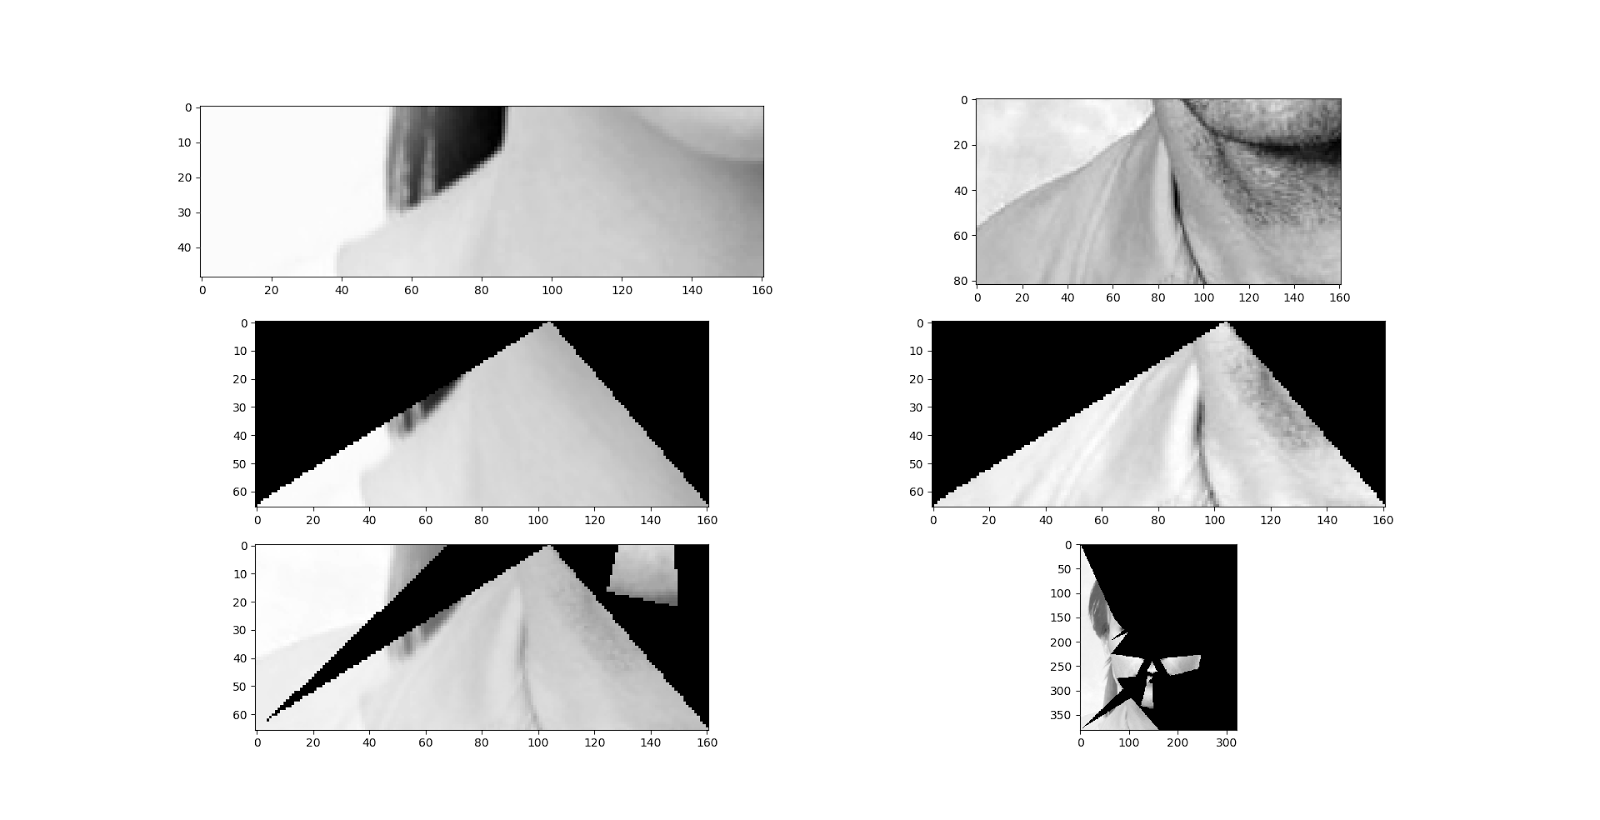
\includegraphics[width = \linewidth]{triangles}
	\caption{Masked Triangles}
\end{figure}


\subsection{GIF Creation}
A GIF, at its most basic, is a series of static images joined and played in series. By pushing each still into a NumPy array, the GIF generated from the array appears to be a seamless morph. The reverse playback can be created by appending the reverse of the image array to itself. Because each frame in a GIF can have an independent duration, a longer pause at the start and end frames should be created to emphasize each original image. Similar to video, creation of a GIF has an inherent tradeoff of filesize and fluidity/frame rate. For our design, we opted for fewer frames (8 frames) because we wanted to service as many server requests as possible. Using Python's imageio, we further quantized the color spectrum to only 32 shades of grey for each frame and create a compressed GIF from that array of frames.

\subsection{Server}
	An in-class demonstration is a desirable goal and it is important that the server works as smooth and efficient as possible. This implies that fast results are desired so that a user does not have to wait for a GIF to be created.We use a simple REST server based on CherryPy with two endpoints. On one, we return static files such as the HTML and CSS of a page. On the other, we accept two images from the user and redirect the user to the static GIF generated from those two images. Each frame of the GIF can be generated independent of other frames, so we decided to parallelize the process. Thus we create a Python pool object to handle the parallelization of frame generation. 



\section{Results}
	The generated GIF results in a seamless transition from image I to J using varying values of alpha to morph the two images. Examples of this transition can be seen in Appendix B. While image morphing and GIF generation seems to perform well on a PC, users may have difficulty with results when accessing the server on a mobile device. If an image depicts a face with glasses, this may also cause problems with the program.  


\section{Conclusion}
In this paper, we provide a framework for implementing Facial Image Morphing using Python, Dlib, and OpenCV. After landmark detection and subdivision, we are able to warp the images to produce a morphed image M. The morphed image can then be manipulated by alpha to show varying degrees of each original image.  By varying the value of alpha we are able to create an array of images that will demonstrate a transition from image I to J and can be viewed as a GIF.

\section{Appendix A: Code}
See \url{https://github.com/conradhappeliv/imagemorpher} for the full code-base and instructions on running.


% conference papers do not normally have an appendix


% use section* for acknowledgement
%\section*{Acknowledgment}


\section{Appendix B: Examples}
\begin{figure*}[!t]\label{fig:merge}
	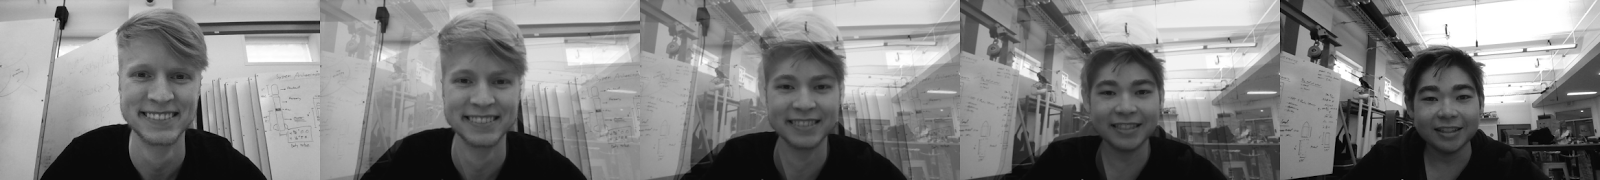
\includegraphics[width = \linewidth]{sample1}
	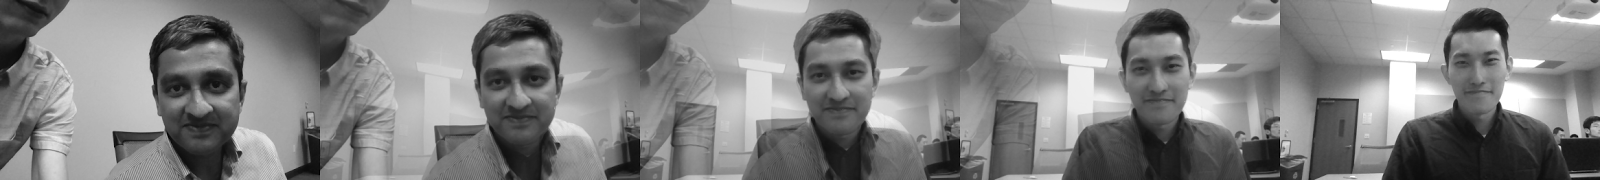
\includegraphics[width = \linewidth]{sample2}
	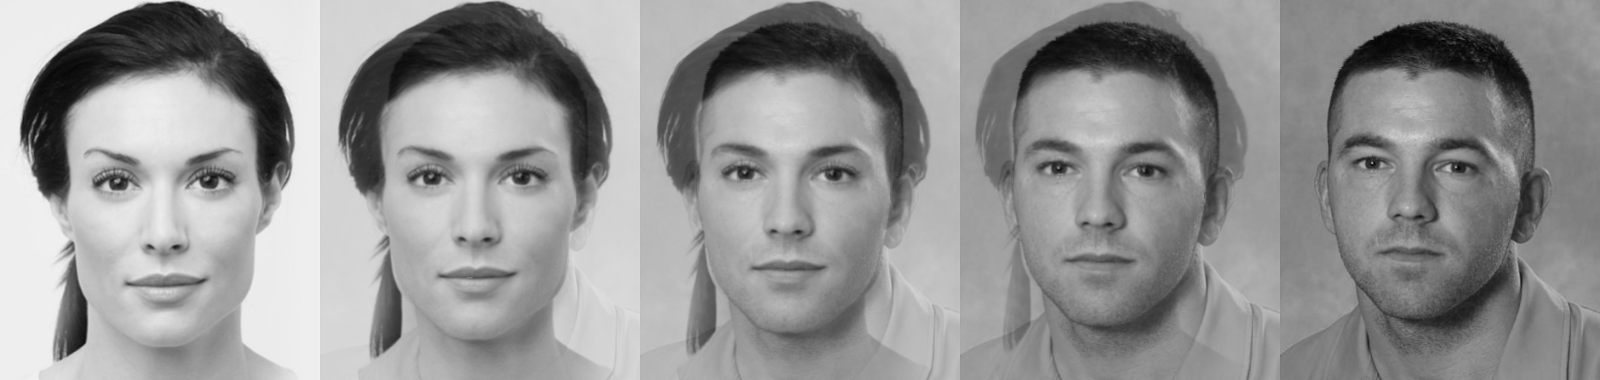
\includegraphics[width = \linewidth]{sample3}
	\caption{Sample Merge Sequences}
\end{figure*}

% that's all folks
\end{document}


